\documentclass{amsart}
\usepackage{fullpage}

\usepackage[T1]{fontenc}
\usepackage[utf8]{inputenc} 
\usepackage{lmodern}
\usepackage[slovene]{babel}
\usepackage{hyperref}
\usepackage{amsmath,amssymb,amsfonts, mathtools}
\usepackage{bbm}
\usepackage{graphicx}
\graphicspath{{./images/}}

\linespread{1.15}

\newcommand{\N}{\mathbb{N}}
\newcommand{\Z}{\mathbb{Z}}
\newcommand{\Q}{\mathbb{Q}}
\newcommand{\R}{\mathbb{R}}
\newcommand{\C}{\mathbb{C}}

% ukazi za matematicna okolja
\theoremstyle{definition} % tekst napisan pokoncno
\newtheorem{definicija}{Definicija}[section]
\newtheorem{primer}[definicija]{Primer}
\newtheorem{opomba}[definicija]{Opomba}

\renewcommand\endprimer{\hfill$\diamondsuit$}

\theoremstyle{plain} % tekst napisan posevno
\newtheorem{lema}[definicija]{Lema}
\newtheorem{izrek}[definicija]{Izrek}
\newtheorem{trditev}[definicija]{Trditev}
\newtheorem{posledica}[definicija]{Posledica}

\title{Kontekstno-neodvisne gramatike za kodiranje in stiskanje podatkov}
\author{Janez Podlogar}
\date{\today}

\begin{document}

\begin{abstract}

    V delu podamo definicje kodiranja, dekodiranja in stiskanja podtakov ter predstavimo
    primere, ki motivirajo stiskanje podatkov s kontekstno-neodvisnimi gramatikami.

\end{abstract}

\maketitle

\section{Kodiranje podatkov}

Zapis informacije v neki obliki ni primeren za vsakršno rabo. Besedilo, zapisano z 
pismenkami, je neberljivo za slepe osebe, saj je komunikacijski kanal v tem primeru
vid. Prav tako pisanega besedila v pravotni obliki ni mogoče poslati s telegrafom. V tem
primeru je komunikacijski kanal žica in pismenke se po njej ne morejo sprehoditi. V obeh 
primerih je informacija, ki bi jo radi prenesli v neprimerni obliki. V prvem 
primeru je potrebno besedilo zapisati z Braillovo pisavo. V drugem primeru pa je
potrebno besedil pretvoriti v električni signal. Spreminjanje zapisa sporočila
imenujemo \textit{kodiranje}, sistemu pravil, po katerem se kodiranje opravi,
pa \textit{kod}. 

\begin{primer}\label{Morse}

    \textit{Morsejeva abeceda} je kodiranje črk, števil in ločil s pomočjo zaporedja kratkih
    in dolgih signalov:

    \begin{itemize}
        \item Dolžina kratkega signala je ena enota.
        \item Dolgi signal je trikrat daljši od kratkega signala.
        \item Razmik med signali znotraj črke je tišina dolžine kratkega signala.
        \item Razmik med črkami je tišina dolga tri kratke signale oz. en dolgi signal.
        \item Presledek med besedami je tišina dolga sedmih kratkih signalov.
    \end{itemize}

    \begin{figure}[h]
        \centering
        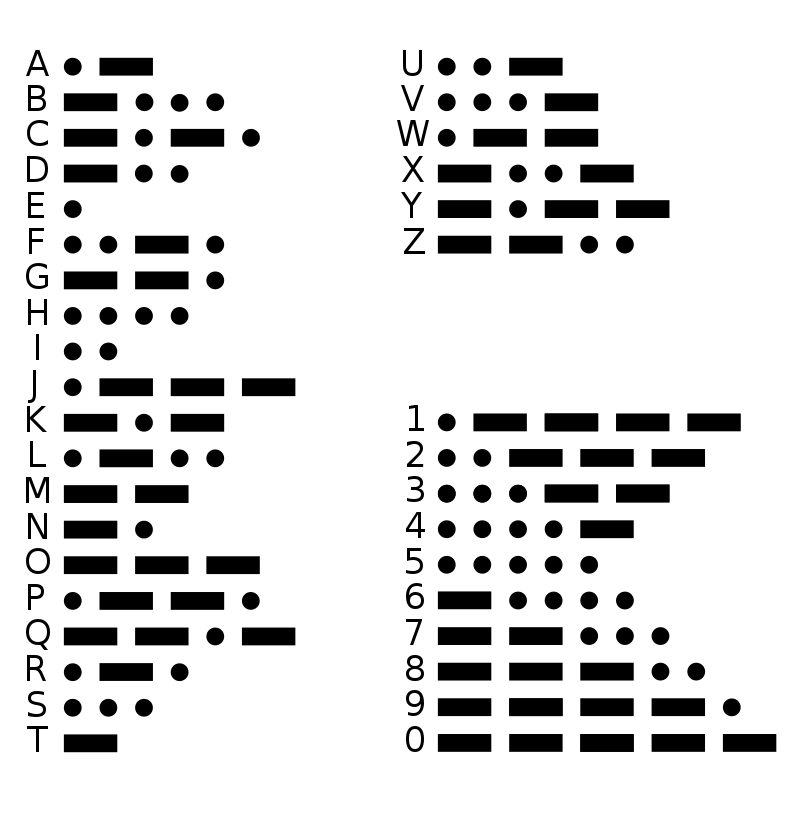
\includegraphics[width=4.3cm]{International_Morse_Code.svg.png}
        \caption{Mednarodna Morsejeva abeceda}
        \label{fig:Morse}
    \end{figure}

    Prvotni namen Morsejeve abecede je komunikacija preko telegrama, saj komunikacijski
    kanal dovoljuje le električne signale in tišino med njimi. Kodiranje črk je takšno,
    da imajo črke z višjo frekvenco (v angleškem jeziku) krajši zapis. Tako se dolžina
    kodiranega sporočila skrajša in posledično tudi čas prenosa.

\end{primer}

\begin{definicija}

    \textit{Abeceda} je končna neprazna množica $ \Sigma $. Elementom abecede pravimo \textit{črke}.
    \textit{Množica vseh končnih nizov abecede} $ \Sigma $ je
    \[
        \Sigma^* = \{ a_1 a_2 a_3 \cdots a_n \mid n \in \N_0 \land \forall i: a_i \in \Sigma \}, 
    \]
    kjer za $ n = 0 $ dobimo prazen niz, ki ga označimo z $ \varepsilon $.
    \textit{Dolžino niza w} označimo z $ |w| $ in je enaka številu črk v nizu $ w \in \Sigma^* $.
    \textit{Jezik na abecedi} $ \Sigma $ je poljubna podmnožica množice $ \Sigma^* $. 

\end{definicija}

\begin{opomba}
    
    \textit{Kleenejeva zvezdica} ali \textit{Kleenejevo zaprtje} je operacija, ki
    abecedi $ \Sigma $ priredi najmanjšo nadmnožico $ \Sigma^* $, ki vsebuje
    \textit{prazen niz} $ \varepsilon $ in je zaprta za konkatenacijo oziroma veriženje.
    Z drugimi besedami, $ \Sigma^* $ je množica vseh končnih nizov, ki
    jih lahko generiramo z veriženjem črk abecede $ \Sigma $. \\
    Za abecedo $ \Sigma $ definirajmo
    \[
        \Sigma^0 = \{ \varepsilon \}, \quad \Sigma^1 = \Sigma
    \]
    ter za vsak $ i > 0 $ rekurzivno
    \[
        \Sigma^{i+1} = \{ wa \mid w \in \Sigma^i \text{ in } a \in \Sigma \}.
    \]
    Potem je Kleenejeva zvezdico na $ \Sigma $ enaka
    \[
        \Sigma^* = \bigcup_{i \geq 0} \Sigma^i.
    \]

\end{opomba}

\begin{primer}
    
    Naj bo $ \Sigma = \{ a,b,c \} $ abeceda, potem je
    \[
        ab \in \Sigma^*, \quad ccc \in \Sigma^*, \quad cababcccababcccab \in \Sigma^*.
    \]

\end{primer}

\begin{definicija}
    
    \textit{Kodiranje nizov abecede} $ \Sigma $ je injektivna funkcija $ \kappa \colon \Sigma^* 
    \to \Sigma_c^* $, kjer je $ \Sigma_c $ \textit{kodirna abeceda} in $ \kappa(w) $ imenujemo
    \textit{koda niza} $ w $. \textit{Dokodiranje kodiranja} $ \kappa $ je funkcija 
    $ \kappa^{-1} \colon C \subseteq \Sigma^*_c \to \Sigma^* $, da velja
    \[
        \forall w \in \Sigma^* \colon \kappa^{-1}(\kappa(w)) = w.
    \]

\end{definicija}

\begin{opomba}
    
    Zožitev kodomene kodirne funkcije $ \kappa $ na $ C \subseteq \Sigma^*_c $ je bijektivna funkcija.

\end{opomba}

\begin{primer}
    
    Formalizirajmo Morsejevo abecedo iz Primera~\refeq{Morse}. Abecedi sta
    \[
        \Sigma = \{ \text{A},  \text{B}, \ldots, \text{Z} \} \cup \{ 0, 1, \ldots, 9 \} \cup \{ \_ \}, \quad
        \Sigma_c = \{ \cdot ,-, \_ \}.
    \]
    Definirajmo kodirno funkcijo črk abecede $ \kappa \colon \Sigma \to \Sigma_c^* $, ki vsaki črki iz abecede
    $ \Sigma $ priredi niz črk kodirne abecede $ \Sigma_c $. Vrednosti funkcije $ \kappa $ so določene s
    tabelo iz Slike~\refeq{fig:Morse}, dodatno presledek med besedami \_  kodiramo v šest kratkih enot tišine 
    \[
        \kappa(\_) = \_\_\_
    \]
    Za niz $ w = a_1a_2 \ldots a_n \in \Sigma^* $ definiramo kodirno 
    funkcijo $ K $ po črkah
    \[
        K(w) = \kappa(a_1)\_\kappa(a_2)\_\cdots\kappa(a_n).
    \]
    Poglejmo si dva primera kodiranja in v Morsejevi abecedi
    % Za tišino med črkami uporabimo presledek \;\;, za tišino med besedami uporabimo presledek \qquad
    \begin{gather*}
        K(\text{SOS}) = \cdot\cdot\cdot \;\; --- \;\; \cdot\cdot\cdot, \\
        K(\text{AD HOC}) = \cdot- \;\; -\cdot\cdot \qquad \cdot\cdot\cdot\cdot \;\; --- \;\; -\cdot-\cdot.
    \end{gather*}
    Recimo, da smo dobili sporočilo, a se je pošiljatelj zmotil in je namesto kode 
    $ --\cdot- \,\, \cdot \,\, -\cdot\cdot $, ki bi se dekodirala v
    \[
        K^{-1}(--\cdot- \,\, \cdot \,\, -\cdot\cdot) = \text{QED},
        \]
    poslali kodo
    \[
        --\cdot-- \,\, \cdot \,\, -\cdot\cdot.
    \]
    Sporočila ne znamo dekodirati, saj se ne nahaja v domeni $ C $ dekodirne funkcije $ K^{-1} $.
    Natančneje ne obstaja dekodiranje signala $ \kappa^{-1}(--\cdot--) $.

\end{primer}

\section{Stiskanje podatkov}

Eden izmed namen kodiranja je tudi doseči čim večjo ekonomičnost zapisa. Želimo, da bi bilo naše sporočilo
čim krajše. Kodiranje, ki skrajša zapis podatkov, imenujemo \textit{stiskanje podatkov}.

\begin{definicija}
    
    \textit{Stiskanje} je kodiranje $ K $ za katerega velja 
    \[ 
    \exists n \in \N \ \forall w \in \Sigma^* \colon |w| \geq n \implies
    \left\lvert K(w)\right\rvert \ll \left\lvert w \right\rvert.
    \]

\end{definicija}

\begin{opomba}
    
    Ločimo \textit{kodiranje brez izgube}, kjer velja
    \[
        \forall w \in \Sigma^* \colon \kappa^{-1}(\kappa(w)) = w
    \]
    in \textit{kodiranje z izgubo}, kjer kodiranje ni reverzibilen proces
    in v grobem velja
    \[
        \forall w \in \Sigma^* \colon \kappa^{-1}(\kappa(w)) \approx w.
    \]

\end{opomba}

\begin{primer}\label{Stiskanje}
    
    Za abecedo vzemimo $ \Sigma = \{ a,b,c \} $ in poglejmo niz
    \[
        w = cababcccababcccab.
    \]
    Opazimo, da se nam v nizu $ w $ večkrat ponovita vzorca $ ab $ in $ ccc $. Zato
    uvedemo novi spremenljivki $ A = ab $ in $ B = ccc $. Sedaj lahko zapišemo $ w $ kot
    \[
        w = cAABAABA.
    \]
    Ponovno se nam pojavi vzorec, tokrat $ AAB $. Uvedemo novo spremeljivko $ C = AAB $
    in zapišemo $ w $ kot
    \[
        w = cCCA.
    \]
    Prvotni niz smo z novimi spremeljivkami skrajšali. Kot bomo videli, smo
    pretvorili niz $ w $ v kontekstno neodvisno gramatiko $ G_w $ s
    produkcijskimi pravili
    \begin{align*}
        & S  \rightarrow  cCCA, \\
        & A  \rightarrow  ab, \\
        & B  \rightarrow  ccc, \\
        & C  \rightarrow  AAB.
    \end{align*}

\end{primer}

\section{Kontekstno-neodvisne gramatike}

\begin{definicija}

    \textit{Formalna gramatika} $ G $ so pravila, ki nam iz abecede $ \Sigma $ tvorijo jezik,
    označimo ga z $ L(G) $.

\end{definicija}

\begin{definicija}

    \textit{Kontektsno-neodvisna gramatika} je četverica $ G = ( V, \Sigma, P, S ) $, kjer je
    $ V $ končna množica \textit{spremenljivk}, abeceda $ \Sigma $ množica \textit{končnih simbolov} tako,
    da $ \Sigma \cap V = \emptyset $, $ P \subseteq V \times ( V \cup \Sigma )^* $ relacija, ki ji
    pravimo \textit{produkcijsko pravilo} in $ S \in V $ \textit{začetna spremenljivka}.

\end{definicija}

\begin{definicija}
    
    Naj bo $ G = ( V, \Sigma, P, S ) $ kontekstno-neodvisna gramatika. Naj bodo $ \alpha $,
    $ \beta $, $ \gamma \in ( V \cup \Sigma )^* $ nizi spremenljivk in končnih simbolov,
    $ A \in V $ spremenljivka ter naj bo $ ( A, \beta ) \in P $ produkcijsko pravilo,
    označimo ga z $ A \rightarrow \beta $. Pravimo, da se $ \alpha A \gamma $ 
    \textit{prepiše s pravilom} $ A $ v $ \alpha\beta\gamma $, pišemo $ \alpha A \gamma  \Rightarrow 
    \alpha\beta\gamma $. Pravimo, da $ \alpha $ \textit{porodi} $ \beta $, če je $ \alpha = \beta $ ali če
    za $ k \geq 0 $ obstaja zaporedje $ \alpha_1, \alpha_2, \ldots \alpha_n
    \in ( V \cup \Sigma )^* $ tako, da 
    \[
        \alpha \Rightarrow \alpha_1 \Rightarrow \alpha_2 \Rightarrow \ldots \Rightarrow \alpha_n
        \Rightarrow \beta
    \]
    in pišemo $ \alpha \xRightarrow{*} \beta $.

\end{definicija}

\begin{posledica}

    Jezik kontekstno neodvisne gramatike $ G $ je
    \[
        L(G) = \{ w \in \Sigma^* \mid S \xRightarrow{*} w \}.
    \]

\end{posledica}

\begin{opomba}
    
    Ime kontekstno-neodvisna gramatika izvira iz oblike produkcijskih pravil. Na levi
    strani produkcijskega pravila mora vedno stati samo spremenljivka. Torej vsebuje samo
    pravila oblike
    \[
        A \rightarrow \alpha,
    \]
    kjer je  $ A \in V $ in $ \alpha \in ( V \cup \Sigma )^* $. Ne sme pa vsebovati
    pravila oblike
    \[
        \alpha A \gamma \rightarrow \alpha\beta\gamma,
    \]
    kjer je $ A \in V $ in so $ \alpha, \beta, \gamma \in ( V \cup \Sigma )^* $, saj je
    pravilo odvisno od predhodnega konteksta. Odvisno je od tega ali pred njim stoji $ \alpha $
    in za njim $ \beta $.

\end{opomba}

\begin{primer}
    
    Formalizirajmo gramatiko iz Primera~\refeq{Stiskanje}, ki smo jo generirali z nizom
    $ w = cababcccababcccab $. Označimo jo z $ G_w = ( V, \Sigma, P, S ) $, kjer je 
    \begin{gather*}
        V = \{ S, A, B, C \}, \\
        \Sigma = \{ a, b, c \}, \\
        P = \{ S  \rightarrow  cCCA, A  \rightarrow  ab, B  
        \rightarrow  ccc, C  \rightarrow  AAB \}, \\
        S = S.
    \end{gather*}
    Vidimo, da $ G_w $ ustreza naši definiciji kontekstno-neodvisne gramatike
    in res kodira $ w $, saj je 
    \[
        L(G_w) = \{w\}.
    \]
    Dolžina gramatike $ G_w $ je enaka številu črk abecede $ \{ S, A, B, C, \rightarrow \} $,
    ki smo jih porabili za opis gramatike in je enaka $ |P| = 20 $. Vidimo, da niza $ w $ 
    nismo skrajšali, saj je $ |w| = 17 $. Niz $ w $ je bil prekratek, da bi ga lahko
    zares stisnili. Naj bo sedaj
    \[
        w =   cababcccababcccabababccc.
    \]
    Gramatika, ki jo generira novi niz se od prejšnje gramatike razlikuje le v
    \[
        P = \{ S  \rightarrow  cCCAC, A  \rightarrow  ab, B  
        \rightarrow  ccc, C  \rightarrow  AAB \}.
    \]
    Sedaj smo stisnili $ w $ z $ G_w $, saj je
    \[
        |w| = 24 > 21 = |P|.
    \]

\end{primer}

Za razliko od klasičnih metod stiskanja, naša metoda ne izvaja procesa stiskanja
direktno na nizu $ w $, temveč poiščemo gramatiko $ G_w $, ki generira 
enojec $ \{ w \} $ za svoj jezik. Med njimi poiščemo ``najmanjšo'', ki jo nato kodiramo.
Ker gramatike $ G_w $ generira $ w $ in ker je gramatika ``majhna'' jo bomo kodirali v 
``kratko'' kodo. Tako bomo preko gramatike ``dobro'' stisnili niz $ w $.

\end{document} 